
\documentclass[10pt]{article}

\linespread{1} 
\usepackage{float}

\usepackage{geometry}
 \geometry{
  papersize={175mm,248mm},
 total={175mm,248mm},
 left=26mm,
 right=13mm,
 bottom=17mm,
 top=13mm,
 }


\usepackage{amsfonts,amssymb,graphicx,color,epstopdf}
\usepackage[font=small,labelfont=bf]{caption}
\usepackage{subcaption}

\usepackage{color, colortbl, framed}
\usepackage[T1]{fontenc}
\usepackage{mathptmx}

\usepackage{amsmath}
%\usepackage{lineno,hyperref}
\usepackage{authblk}
\usepackage{titlesec}
\usepackage{eucal}
%\DeclareMathAlphabet{\mathpzc}{OT1}{pzc}{m}{it}
%\usepackage{epstopdf}

\usepackage{hhline}
\usepackage{xcolor,colortbl}
\renewcommand{\figurename}{Fig.}

%  \setcounter{secnumdepth}{0}
\usepackage{titlesec}
\titlespacing{\section}{0pt}{\parskip}{-\parskip}
\titlespacing{\subsection}{0pt}{\parskip}{-\parskip}
 \titleformat*{\section}{\normalfont\fontfamily{ptm}\fontsize{10}{19}\bfseries}
 \titleformat*{\subsection}{\normalfont\fontfamily{ptm}\fontsize{10}{18}\bfseries}


\usepackage[sort&compress,square]{natbib}
\setlength{\bibsep}{0.0pt}


\usepackage{authblk}
\usepackage{varwidth}

\renewcommand*{\Authsep}{, }
\renewcommand*{\Authand}{, }
\renewcommand*{\Authands}{, }
\renewcommand*{\Affilfont}{\normalsize\normalfont}
\renewcommand*{\Authfont}{\normalsize\normalfont\bfseries}
\setlength{\affilsep}{0em}

\renewcommand{\abstractname}{}    % clear the title
\makeatletter
\renewcommand{\maketitle}{\bgroup\setlength{\parindent}{0pt}
\begin{flushleft}
  \textbf{\@title}
\vspace{10pt}

  \@author
\end{flushleft}\egroup
}
\makeatother

\title{\fontsize{16pt}{10pt}\selectfont\flushleft \textbf{Mobile based vibration monitoring and its application to road quality monitoring in deep underground mine}}
\author[1]{Radoslaw Zimroz}
\author[1]{Jacek Wodecki}
\author[1]{Justyna Hebda-Sobkowicz}
\author[2]{Agnieszka Wy{\l}oma{\'n}ska}
\author[2]{Pawe{\l} Stefaniak}
\author[3]{Pawe{\l} {\'S}liwi{\'n}ski}
\author[3]{Tomasz Kaniewski}

\affil[1]{Faculty of Geoengineering Mining and Geology, Wroclaw University of Science and Technology, Na Grobli 15, 50-421 Wroclaw}
\affil[2]{KGHM Cuprum Ltd, Research and Development Centre, Sikorskiego 2-8, 53-659 Wroclaw, Poland}
\affil[3]{KGHM Polish Copper, Lubin, Poland
\protect\\
\textbf{E-mail:}{\{radoslaw.zimroz, jacek.wodecki, justyna.hebda-sobkowicz \}@pwr.edu.pl, \{awylomanska,pkstefaniak\}@cuprum.wroc.pl, \{pawel.sliwinski, tomasz.kaniewski\}@kghm.com}}

\date{} 

\begin{document}
\maketitle
\textbf{Abstract.} Road quality is an important issue in everyday life for all car owners. This issue seems to be critically important in underground mines, where LHD machines are used for material transport. One of the biggest problem for LHD operation is relatively quick tires degradation. One of possible reasons might be road surface quality, indeed. However, driver's skills as well as ways of machine operation (loading, acceleration, breaking...) might also play a crucial role. Nowadays, many of machines are equipped with onboard monitoring system that allows to monitor basic parameters (speed, torque, temperatures, pressures etc) at some predefined components. To complete the picture, we propose to use proposed already (but not for mining applications) vibration measurement for road roughness evaluation. To measure vibration acceleration is relatively easy task (we used simple smartphone here), unfortunately method of parametrization and concluding about road quality is still a challenge in mining case. In this paper we have presented a short communication related to first experimental work and some ideas how to deal with this problem using statistical tools for signal modeling.
\newline \newline
\textbf{Keywords:} road surface quality, vibration monitoring, statistical parametrization, LHD machines, underground mine.

\section{Introduction}

In deep mines horizontal wheeled transportation assets (i.e. load-haul-dump machines, hauling trucks, crew transportation trucks etc.) play key role in gaining productivity of the entire facility. They are designed to work in harsh mining conditions (high temperature, humidity, dust and salinity) and high load-operation \cite{wodecki2018technical,wylomanska2014signal,gustafson2013influence}. Efficiency oriented operation of loaders is main cause of their short total life time (${\sim}$3-4 years). Developed monitoring system leads to identification of main causes of failure events by allowing to follow operational parameters and to perform much more advanced context analysis \cite{wodecki2018technical,zimroz2014self}. However, beside typical condition-monitoring-related approach to manage the fleet, there are other areas of interest, that are potent for analysis and viable for efficiency optimization from the management point of view. One of such areas is the assessment of the road quality  \cite{juska2009analysis, forslof2014continuous, astarita2012mobile, tai2010automatic, sandberg1990road, eriksson2008pothole, wang2018road}. In this paper we would like to adress this problem in deep mine conditions. As it was stated, the effectiveness of the wheeled transportation operation is one of the most important areas for optimization in the underground mine. Road quality monitoring is necessary for the safety reasons, because the vehicles require the acceptable level of road quality to move along the corridors without any problems originating from the road state. It is especially important for evacuation routes and more frequently used haulage paths. The other aspect is related to the maintenance of the machines themselves. It is impossible to guarantee that drivers will always perform carefully enough to ensure machine wear minimization. Proper road surface maintenance can help to prolong the lifespan of crucial components related to driving, or even the entire machine. Finally, there is also a functionality concern. If the road is too uneven or too steep, machine operator has to drive slower, which directly impacts the haulage efficiency as a whole, resulting in less effective production.

\section{Methodology}
Proposed methodology is based on statistical parameterization of piece-wise consistent parts of the route. Hence proper segmentation procedure is necessary for initial extraction of such parts. While in final implementation of such analytical system it would be crucial to apply robust method to split apart the route parts, in this example it was performed manually because of relatively small amount of the data, especially taking into consideration that for presented case study segmentation itself is not a key part.

Segments have been analyzed comparatively and classified into two groups: road segments of good and bad condition. As a first tool for the analysis authors propose to use boxplots to observe the most important statistical parameters like median, quartiles distribution and statistical outliers. Secondly, data distributions within segments are modeled with smoothed histograms to visually observe the differences between the classes.
In this work segmentation has been done manually, however in future work we plan to do segmentation automatically\cite{wodecki2018technical, kucharczyk2017structural, hossa2017automatic, wylomanska2014signal, wylomanska2016impulsive}

\section{Application to acquired data}

Testing phase has been divided into two parts: test in controlled conditions using the well-known surface road performed with the ordinary car, and in-situ test in deep mine where the exact features of the route were unknown. Based on statistical analysis of the data registered during first test, authors attempt to apply the same methodology in order to distinguish varying features of the underground road.

Since proposed methodology is based on vibration data analysis, in both tests a regular smartphone equipped with the 3-axial accelerometer was used. Since in such empirical conditions there is no possibility to place the phone perfectly orthogonally relative to the surface of the Earth for the entire duration of the measurement, the analysis is performed using the vector of energy of vibrations rather than one of the individual axes. This approach is also more appropriate, since it describes the actual vibration amplitudes, omitting the meaning of the axes orientation in three-dimensional space and aggregating the informativeness from all of them.

\subsection{Test in controlled conditions}

\begin{figure}[ht!]
\centering
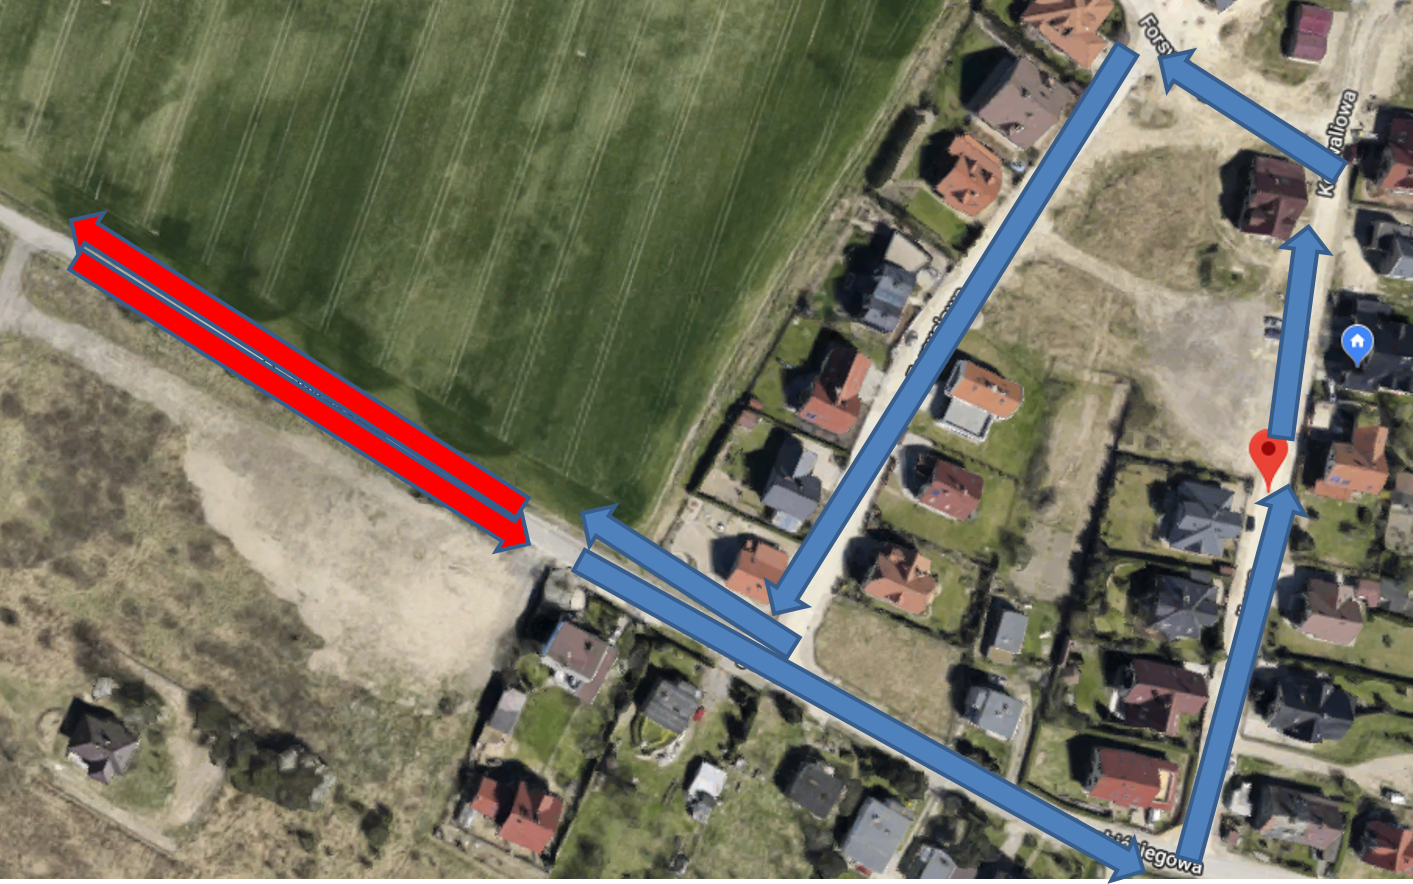
\includegraphics[width=0.7\textwidth]{wykresy/mapa.png}
\caption{A schematic diagram experiment on the surface (poor and good quality of road surface)}
\label{fig:mapa}
\end{figure}

\begin{figure}[ht!]
\centering
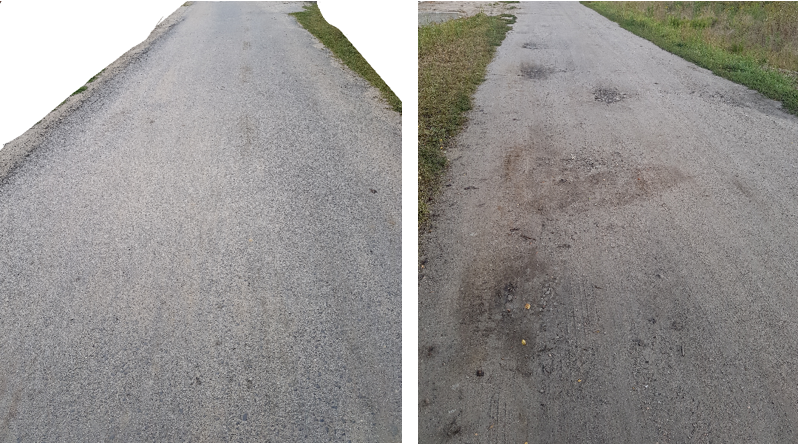
\includegraphics[width=0.7\textwidth]{wykresy/droga.png}
\caption{Photos of good (left) and bad (right) condition road surface used in the test}
\label{fig:droga}
\end{figure}
First test was performed by one of the authors at the local countryside road in Poland (see Fig. \ref{fig:mapa}). Part of the route marked with blue arrows had relatively even asphalt surface, while part marked with red arrows was an uneven dusty country road. Red pin marks the beginning and end of the test route. Quality of road segments are presented in Fig. \ref{fig:droga}.
Phone was placed relatively orthogonally to the car axes (see Fig. \ref{fig:car}). Records of three separate axes of the measurement are presented in the Fig. \ref{fig:raw}. Key driving events have been marked on the signal in the top panel.

\begin{figure}[ht!]
\centering
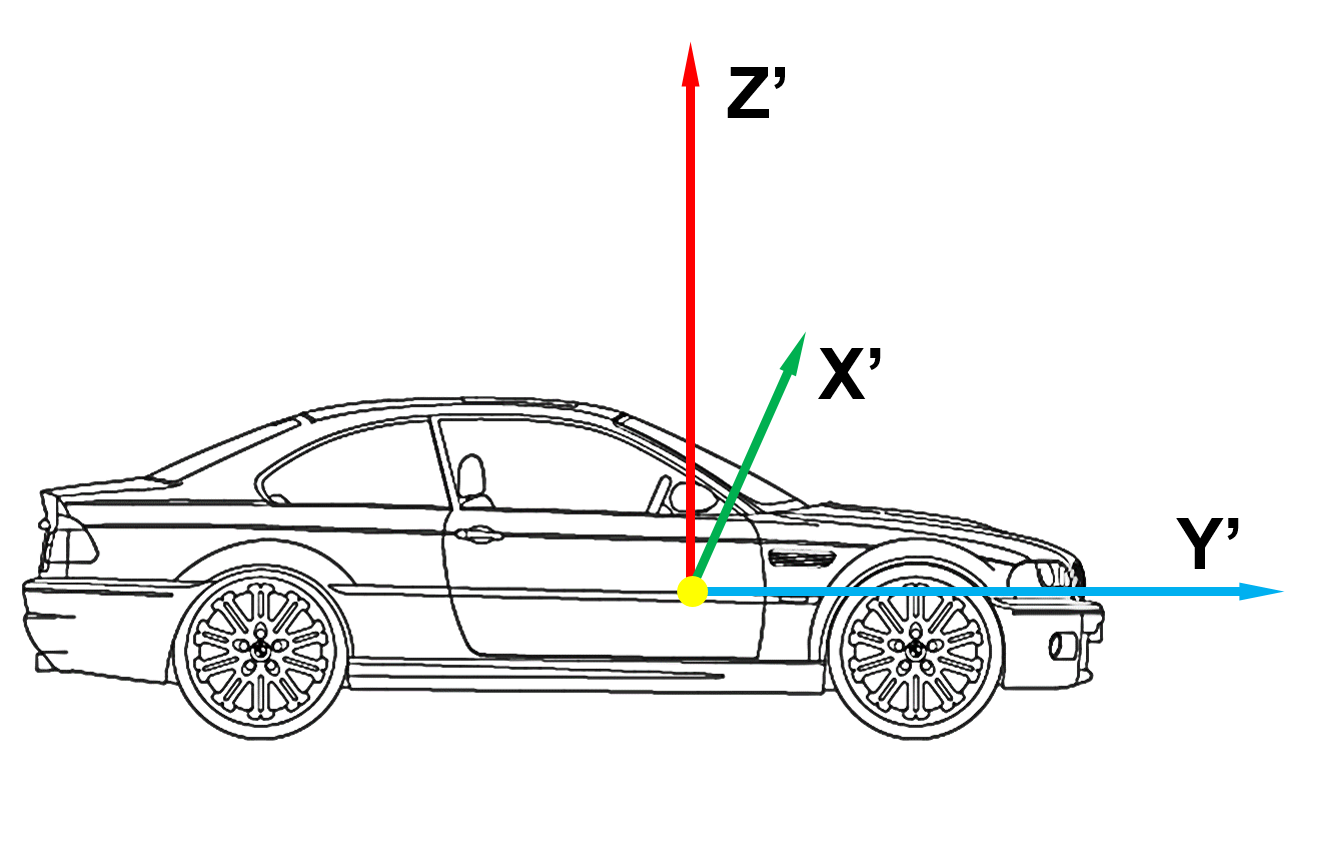
\includegraphics[width=0.6\textwidth]{wykresy/car.png}
\caption{Sensor location during experiment in the car (experiment on surface)}
\label{fig:car}
\end{figure}

\begin{figure}[ht!]
\centering
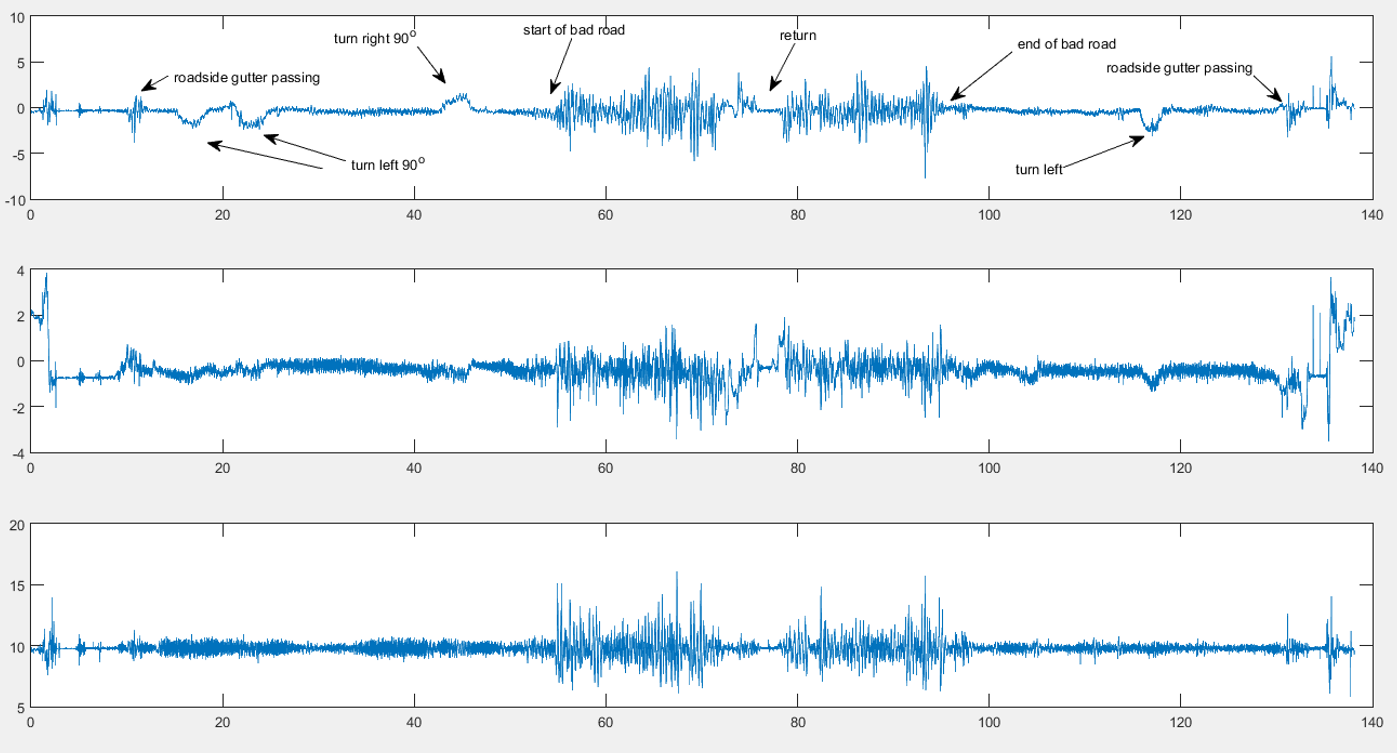
\includegraphics[width=\textwidth]{wykresy/raw.png}
\caption{An example of real data measured on the surface -- controlled conditions}
\label{fig:raw}
\end{figure}

In a first step signal has been segmented manually (see Fig. \ref{fig:seg}). Since in this case road conditions are known, segments have been classified into two classes: good quality road (marked as green) and bad quality road (marked as red). For the purpose of this analysis the moments of taking turns have been omitted.

\begin{figure}[ht!]
\centering
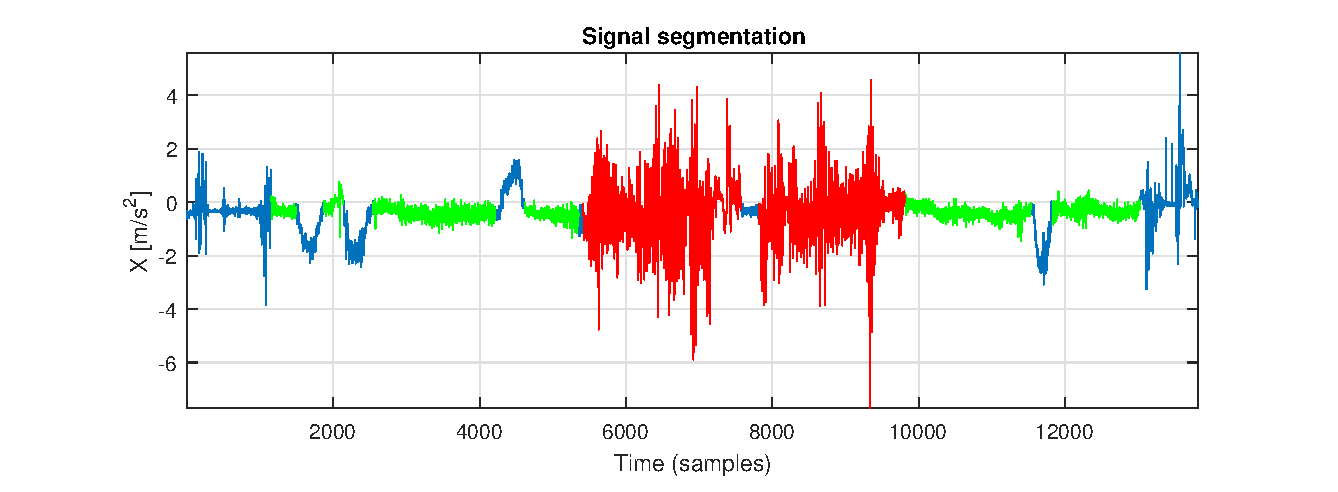
\includegraphics[width=0.8\textwidth]{wykresy/Seg.eps}
\caption{Segmented vibration data}
\label{fig:seg}
\end{figure}

Fig. \ref{fig:stat} presents the results of the comparative analysis. Left panels show both classes as overlapped segments in time domain, which visualizes the differences in vibration energy. In the center panels one can see the boxplots for six segments of good quality road (center top) and two segments of bad quality road (center bottom). Finally, right panels present the empirical distributions modeled as smoothed histograms. One an clearly see the difference between classes in terms of statistical dispersion. On the other hand boxplots as well as distributions show that within individual classes there is high level of similarity between the individual segments. Such clear distinction will serve as a model dataset for the interpretation of the results obtained for the second test.

\begin{figure}[ht!]
\centering
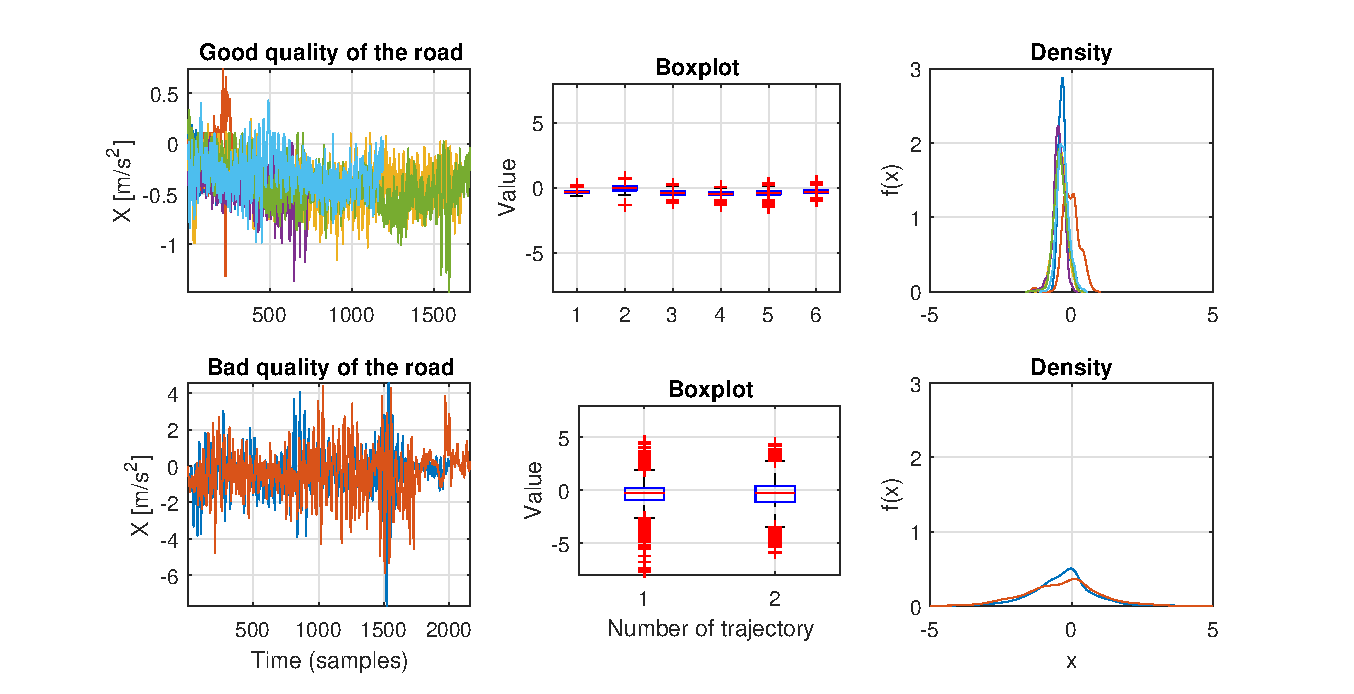
\includegraphics[width=\textwidth]{wykresy/stat.eps}
\caption{Statistical parameterization of the segments.}
\label{fig:stat}
\end{figure}

\subsection{Test in deep mine}

The second test has been performed in one of polish underground mines with standard truck used for crew transportation (see Fig. \ref{fig:truck}). Visual example of the different road qualities is presented in Fig. \ref{fig:droga2}. Raw signals and segmented data are presented in Fig. \ref{fig:raw2} and Fig. \ref{fig:seg2} respectively.

\begin{figure}[ht!]
\centering
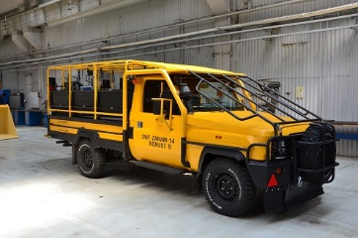
\includegraphics[width=0.5\textwidth]{wykresy/truck.png}
\caption{Investigated crew transportation truck}
\label{fig:truck}
\end{figure}

\begin{figure}[ht!]
\centering
\includegraphics[width=\textwidth]{wykresy/droga2.png}
\caption{Photos of good (left) and bad (right) condition road surface in the underground mine}
\label{fig:droga2}
\end{figure}

\begin{figure}[ht!]
\centering
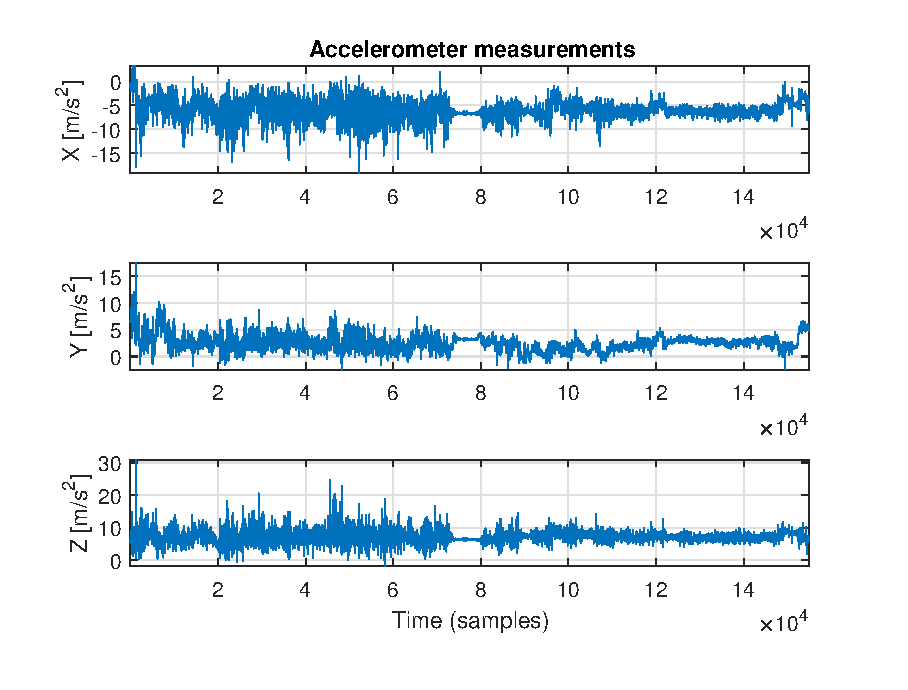
\includegraphics[width=0.7\textwidth]{wykresy/raw2.eps}
\caption{An example of real data measured in the mine}
\label{fig:raw2}
\end{figure}

\begin{figure}[ht!]
\centering
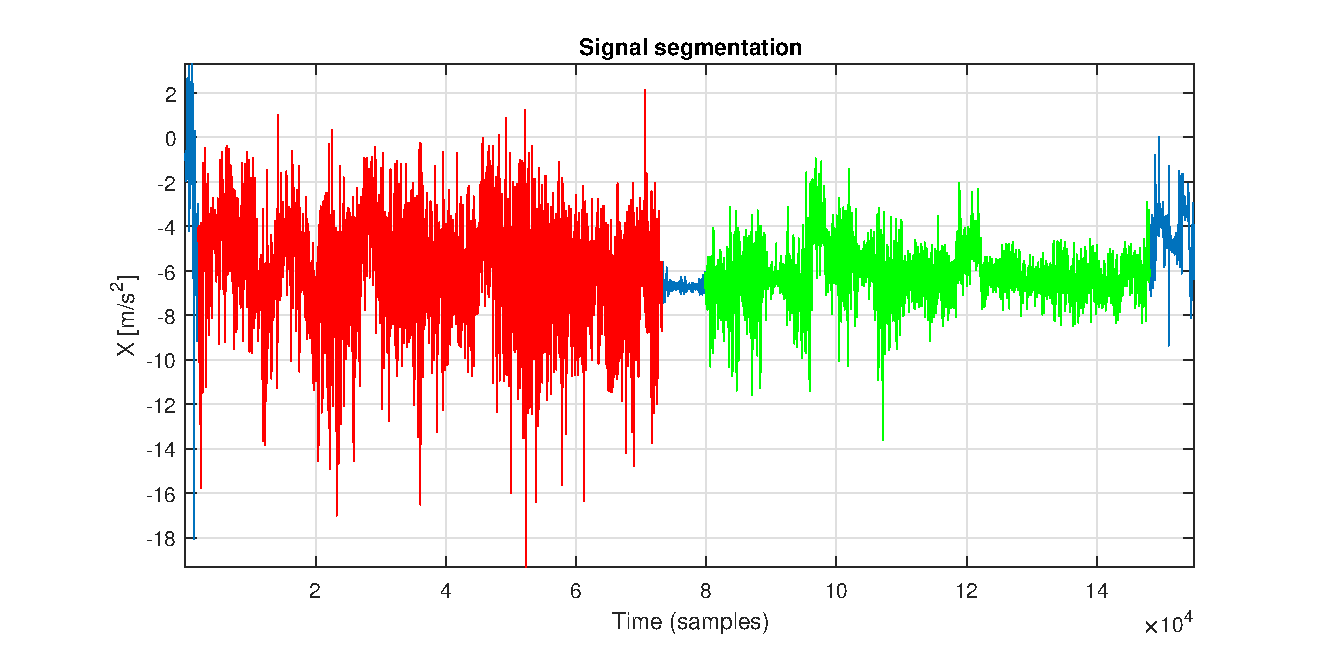
\includegraphics[width=\textwidth]{wykresy/Seg2.eps}
\caption{Segmented vibration data}
\label{fig:seg2}
\end{figure}

Similarly to the first test, results have been presented in terms of time series, boxplots and distributions, however for this dataset only one of each segments is available. Although the difference between the classes may not be as obvious on the time series, boxplots show smaller distance between quartiles as well as tighter spread of the outliers for the road segment of better quality. Empirical distribution of data for better quality segment is clearly more focused around the mode value and clearly distinguishable from the one from the second class. 

\begin{figure}[ht!]
\centering
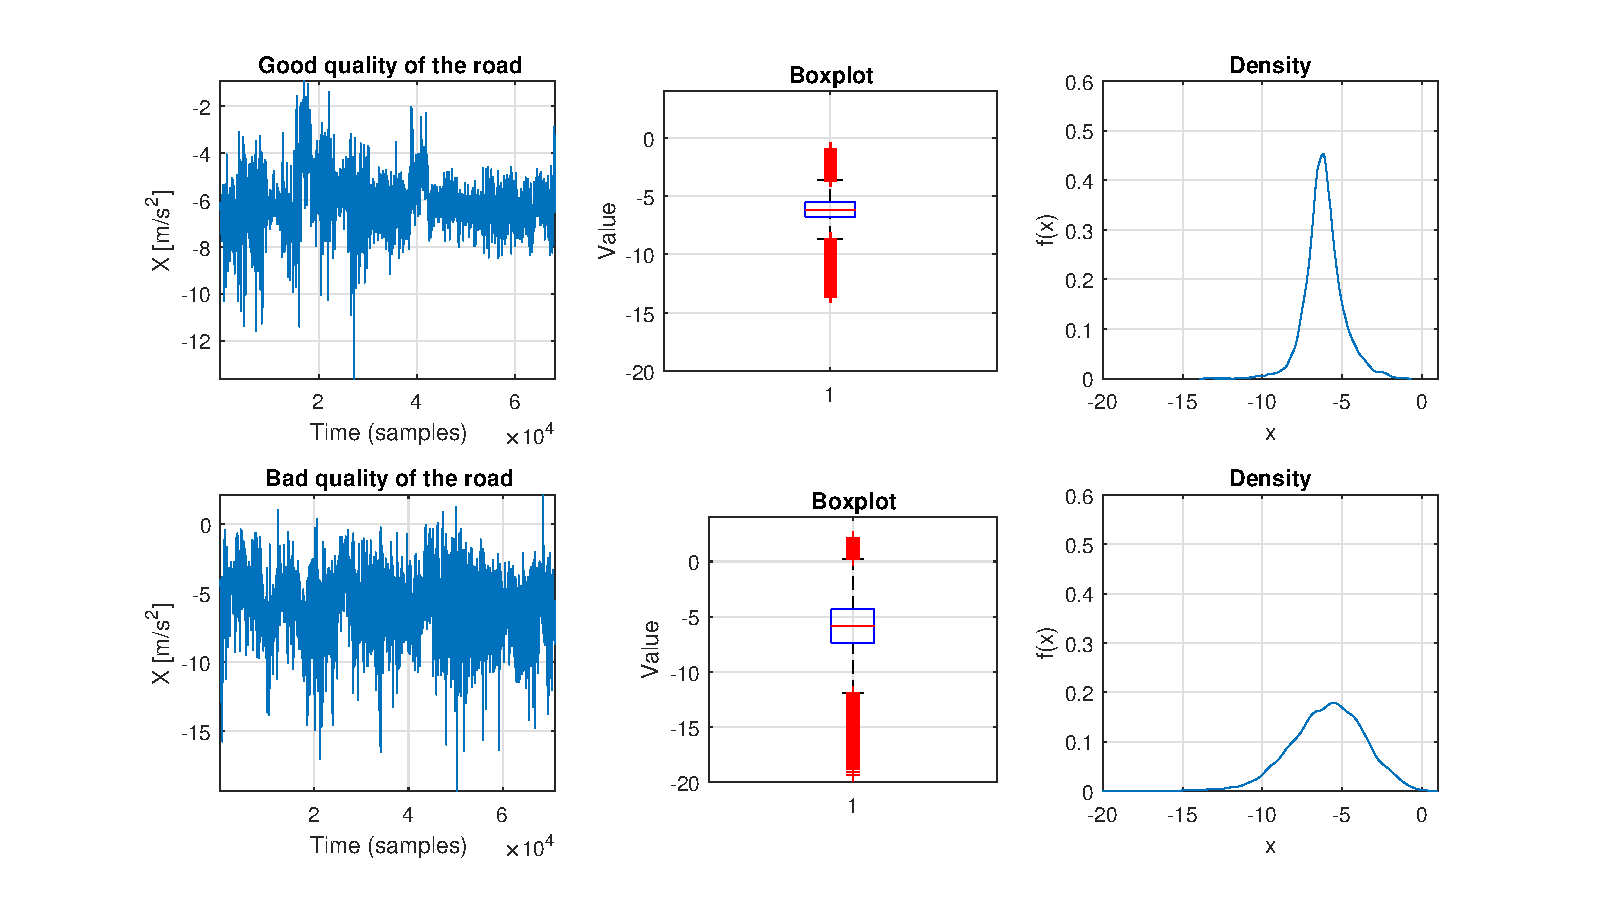
\includegraphics[width=\textwidth]{wykresy/stat2.eps}
\caption{Statistical parameterization of the segments for the second test.}
\label{fig:stat2}
\end{figure}

\section{Conclusions}
In this article, authors have proposed a simple yet robust approach to road quality monitoring in the real-life conditions of the underground mine. Results indicate that simple statistical parameterization allows to distinguish different states of the road surface. Although the amount of road segments was relatively small, first test presents the high level of self-similarity within the classes as well as clearly visible differences between them. The second test confirms the assumption regarding the possibility of assessment and evaluation of the road conditions, which will be also more confident for larger data samples in the future.
\section*{Acknowledgments}
The work of J.Wodecki and J.Hebda-Sobkowicz was supported by the statutory grant.
\bibliographystyle{style}
\bibliography{mybibfile}

\end{document}